\chapter{Scenarios View}

\begin{figure}[ht]
\begin{center}
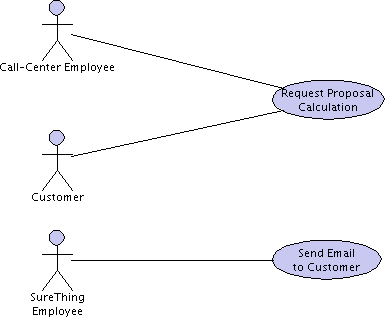
\includegraphics[width=2.5in]{img/uc.png}
\end{center}
\caption{Illustration of representative use cases}
\label{fig:uc}
\end{figure}

This view is a guide through the previous four views (Logical, Process, Development and Physical)
as it shows how a set of use cases which are representative for the system (see figure \ref{fig:uc})
can be carried out in this architecture.

\section{Scenario: Request for proposal calculation}

A use case which we see as relevant for this system, both in terms of coverage of architectural
components and in terms of the frequency with which it appears in real-life is the request issued
by either a Call-Center employee or by a customer for a proposal calculation.

This use case is defined as follows:
\begin{center}
\framebox[4in]{
\begin{minipage}[c]{3.5in}
Use case: Request proposal calculation
\\
Level: User goal
\\
Primary Actor: Call-Center Employee / Customer
\\
\begin{enumerate}
\item Customer requests proposal calculation.
\item System gathers data needed for calculation from the customer.
\item System communicates data over the network to the company's central server.
\item Central server gets request for proposal calculation, performs it and:
\begin{enumerate}
\item stores the result into the database;
\item sends the result back to the requesting customer.
\end{enumerate}
\item System running on customer's host displays proposal to the client.
\end{enumerate}
\end{minipage}}
\end{center}
The way this use case's functionality is achieved differs form one evolutionary phase to the next. All
views cover the system in each of these phases, making it clear what phase each diagram refers to.
Therefore, it is advisable, when working on phase \tt{x}\normalfont, to read the part describing phase
 \tt{x}\normalfont\ from each of the views.

Analysis can begin with the logical view, which makes clear what components of the system are involved
in dealing with this use case. In phase 1, for example, you can see in figure \ref{fig:logical_phase1} that the action
is initiated by the GUI and client UCIS component running on the Call-Center employee's computer, then
the request goes to the central UCIS server, where it is then forwarded (after some possible processing)
to the STIFF system by means of the STIFF Wrapper. Looking at the process view can be particularly
useful here in order to understand how the STIFF Wrapper achieves communication with the STIFF system
itself and is then able to provide the result back to the UCIS system. Naturally, the result is stored (as
specified) in the database, and also sent back to the client UCIS component and displayed on screen.

If you are interested in understanding how the use case is handled in phase 2, you should consult the
logical and process views to notice how the UCIS system is now modified in order to allow web-access.
The use case now is initiated by means of the customer
accessing a certain proposal calculation request web page and making an HTTP request to the central UCIS
system. The logical view shows how the client UCIS component disappears and it is replaced by a
streamline web browser, while the UCIS server is modified so that it now includes all the previously
shared functionality in a form suited for use as a web application. Thus, the central server, which is the
one handling the customer's request, is now accessed as Java servlet processing a HTTP request. The diagram
from figure \ref{fig:pi_2} of the process view shows how the \textit{Front Controller} pattern is employed in order
to dispatch the customer's request to a particular component of the UCIS server. The processing from here on
proceeds in more or less the same way as in phase 1 and you are therefore referred to the explanation of
this phase. In direct connection with this use case is also the physical view, which helps you understand how
the system should be set up in order to function in a web environment capable of handling use cases like
this one.

Finally, for running the use case in phase 3 (the final development phase), proceed in the same way as for
phase 2 up to the point where a request has to be made to the STIFF system and then examine the logical
view of phase 3 to understand the changes made to the STIFF system. The final part of the use case
implies the actual computation of the proposal, preferably in real-time. Here's where the process view
(section \ref{sec:pv_stiff}) and the physical view come into play to give you a clearer image of how the
STIFF system can be distributed in
order to provide real-time response to requests for proposal calculations, even as the number of simultaneous
requests increases. The logical view will also show that the ProD has been, by the end of this phase, moved
to the Oracle database, so STIFF now can get all the data necessary for its computation directly from the
this database.

The development view will not be of particular use for understanding how this use case itself can be realized,
but it will be of help to guide development in such a way that the handling of the use case in each evolutionary
phase brings an additional performance increase. The development view will explain the rationale behind the
decisions to split the development process in the way in which it has been split and it will also explain
why certain development steps have been included in a certain phase and not in another one. Thus, the
development view will be of interest especially to the developers which have to understand the sequence
in which various components that play a part in the realization of this use case have to be modified or
extended.

\section{Scenario: Send email to customer}

The second use case which we see as significant for our architecture is tied only to the last phase of development,
when the so-called GOC (Generic Output Component) is introduced into the system. This use case deals with
a request made by an employee of the SureThing company for an email to be sent to a customer. The contents
of the email is irrelevant (it could be anything from an invoice to a claim handling solution). Also, the form
of the message (i.e., email) is irrelevant as well as it could be any other of the forms provided by the GOC
component (fax, paper and so on). Finally, the addressee (i.e., the customer) is also just an example as it could
very well replaced with another employee of the company, for instance. In light of these facts, a more generic
name for this use case could perhaps be ``Send message to some recipient.''

This definition of this use case is provided below:
\begin{center}
\framebox[4in]{
\begin{minipage}[c]{3.5in}
Use case: Send email to customer
\\
Level: User goal
\\
Primary Actor: Company Employee
\\
\begin{enumerate}
\item Employee requests (usu. by means of either the PROFI or the UCIS system) that an email containing some
relevant information be sent to a customer. As an alternative, the system could generate a request of this kind
itself, as a result of some (e.g.) checks.
\item The system forwards the request, together with the contents of the email, to the GOC component.
\item The system indicates that the requested means of communication is email.
\item The GOC component complies and sends the email to the customer.
\item The GOC component informs the system of the result (success/failure) of the request.
\item The system notifies the employee about the result of its request.
\end{enumerate}
\end{minipage}}
\end{center}

As mentioned already, this use case only relates to the system after the 3\textsuperscript{rd} phase of development,
so you are directed solely to the part of each view which describe this phase. The logical view will show that the
only two systems directly connected to the GOC component are the UCIS and the PROFI systems, which means
that should a request for output be possible from the CHIPS or BuRP subsystems, it would have to go through UCIS.
The development of GOC is beyond the scope of this architectural description (as the component will be provided
``as is'' by a 3\textsuperscript{rd} party), and therefore you will not find detailed information about its inner structure
herein. What both the process view and the logical view will imply with respect to this use case is that PROFI, as well
as UCIS, will have been changed in such a way that they no longer use their own modules for producing output, but
rather that they interface with GOC and forward all such requests to it. Consult the physical
view if you are interested in the actual hardware on which the GOC will be deployed. This will probably concern you
if you are the one installing this component in the system.